%==============================================================================
\chapter{3D biophysical model of biventricular rat heart contraction 
mechanics}\label{cha:chapter02}
%==============================================================================
%
%
%
\begin{remark}{Outline}
    In this chapter, we systematically build a mathematical model of $3$D biventricular rat heart contraction mechanics. We start with modelling ion fluxes across each cell membrane using an ionic model for left ventricular myocytes at physiological temperature and pacing rate (Section~\ref{sec:ch2ionicmodel}). We then model active tension generation at the cellular level using a model of sarcomere contraction, which includes length- and velocity-tension dependencies (Section~\ref{sec:ch2contractionmodel}). We present the framework to build a $3$D computer representation (mesh) of rat biventricular anatomies from experimental data (Section~\ref{sec:ch2anatomy}). We finally describe passive material properties (Section~\ref{sec:ch2tissuemodel}), myocardial electrical activation (Section~\ref{sec:ch2electricalactivation}) and spatial and haemodynamic boundary conditions (Section~\ref{sec:ch2boundaryconditions}). We conclude with a brief summary (Section~\ref{sec:ch2summary}).
\end{remark}

\begin{figure}[ht!]
    \myfloatalign
    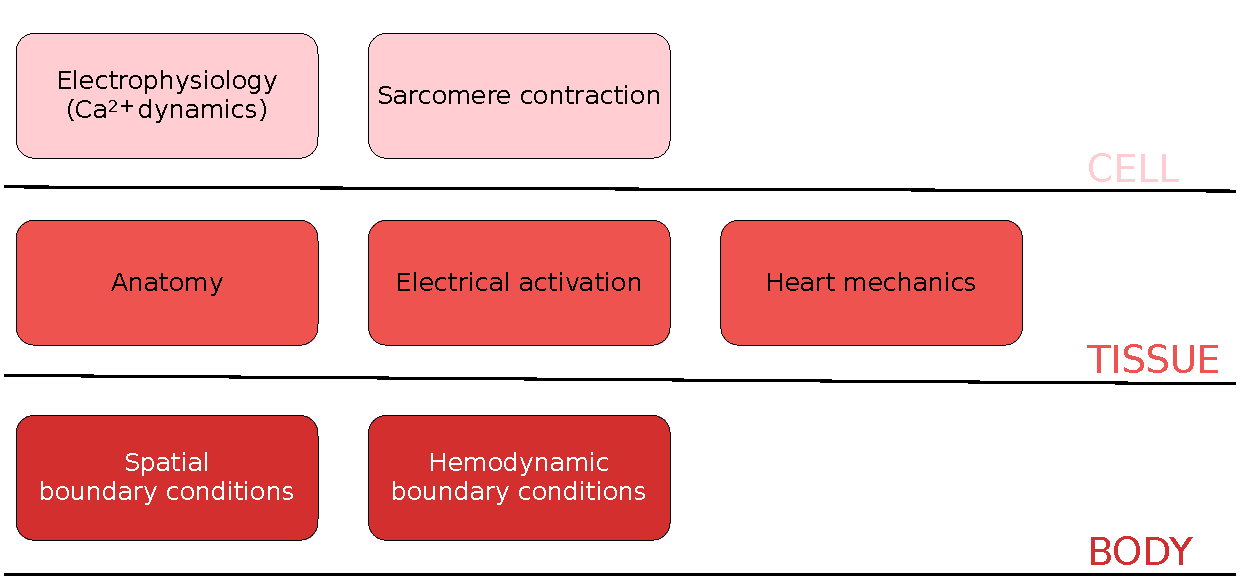
\includegraphics[width=\textwidth]{figures/chapter02/methods_schematic.pdf}
    \caption{The full $3$D biophysical model of biventricular rat heart contraction mechanics is a multi-scale framework of integrated sub-models describing the main mechanisms which regulate the heart contraction and relaxation at the cell, tissue and body scales.}
    \label{fig:methodssummaryinscale}
\end{figure}


%
%
%
\section{Ionic model}\label{sec:ch2ionicmodel}
We employed the Gattoni et al.~\cite{Gattoni:2016} model to simulate rat left ventricular myocytes electrophysiology and calcium dynamics at physiological pacing rate ($\SI{6}{\hertz}$) and temperature ($\SI{37}{\celsius}$). All the currents present in this model are summarised in Table~\ref{tab:gattonicurrentstab}, while the main ion channels, transporters and pumps are depicted in Figure~\ref{fig:gattonicurrentsfig}.

\begin{table}[ht!]
    \myfloatalign
    \begin{tabularx}{\textwidth}{lX}
    \toprule
    \tableheadline{Label} & \tableheadline{Definition} \\
    \midrule
    $I_{LCC}$    & L-type $\Ca$ current \\
    $I_{RyR}$    & ryanodine receptor current \\
    $I_{TRPN}$   & troponin buffering current \\
    $I_{SERCA}$  & sarcoplasmic $\Ca$ pump current \\
    $I_{SR\ell}$ & sarcoplasmic reticulum leakage current \\
    $I_{NCX}$    & $\Na$/$\Ca$ exchanger current \\
    $I_{PMCa}$   & plasma membrane $\Ca$ pump current \\
    $I_{Cab}$    & $\Ca$ leak current \\
    $I_{NaK}$    & $\Na$/$\K$ pump current \\
    $I_{Na}$     & $\Na$ current \\
    $I_{K1}$     & inwardly rectifying $\K$ current \\
    $I_{to}$     & transient outward $\K$ current \\
    $I_{ss}$     & steady-state outward $\K$ current \\
    $I_{f}$      & hyperpolarisation-activated current \\
    $I_{BNa}$    & $\Na$ background current \\
    $I_{BK}$     & $\K$ background current \\
    \bottomrule
    \end{tabularx}
    \caption{Gattoni et al.~\cite{Gattoni:2017} model's ionic currents.}
    \label{tab:gattonicurrentstab}
\end{table}

\begin{figure}[ht!]
    \myfloatalign
    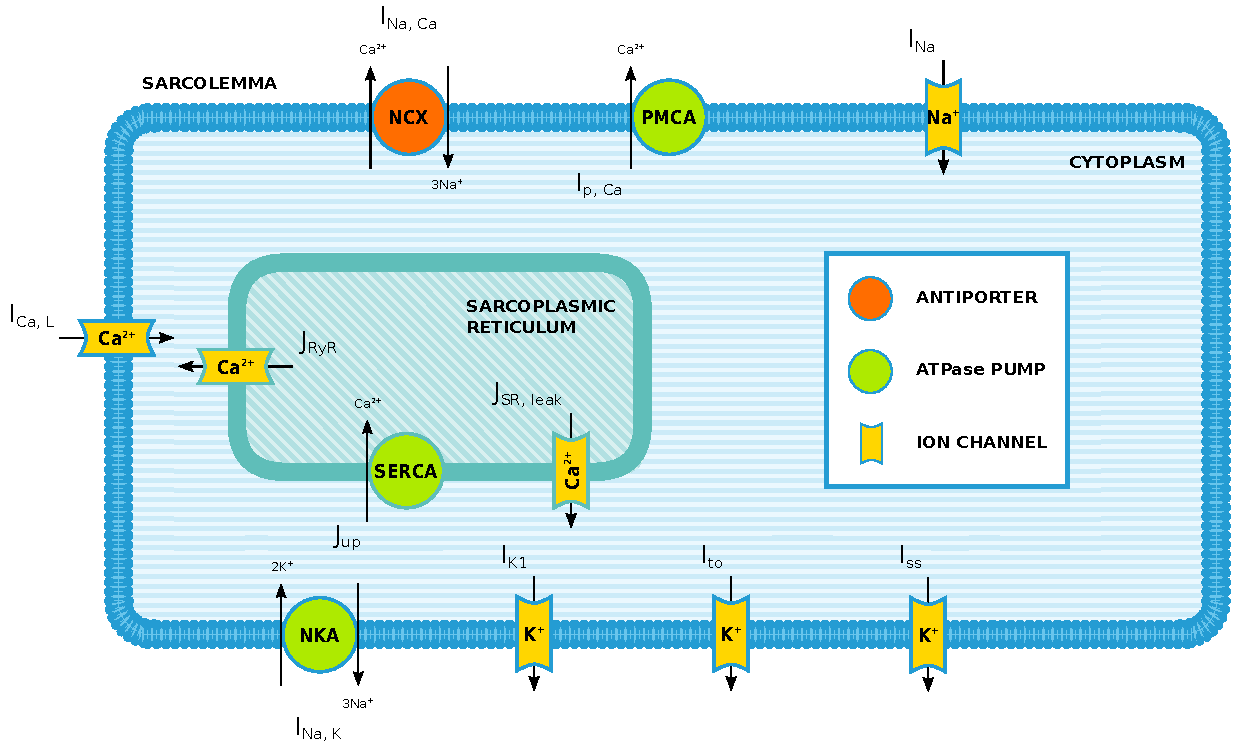
\includegraphics[width=\textwidth]{figures/chapter02/new_ep.pdf}
    \caption{Main ion channels and pumps included in the Gattoni et al.~\cite{Gattoni:2016} model.}
    \label{fig:gattonicurrentsfig}
\end{figure}


%
%
%
\section{Contraction model}\label{sec:ch2contractionmodel}
We employed the Land et al.~\cite{Land:2012} myocyte contraction model to simulate both dynamic force generation at the sarcomere level in response to a calcium transient and the steady-state force-calcium relationship in the rat heart. This model describes the cooperative binding of $\Ca$ to TnC, which causes unblocking of the actin sites for myosin cross-bridge cycling.

\vspace{0.2cm}
The process of $\Ca$ binding to TnC is described via the following equation:
%
\begin{equation}\label{eq:landodesys1}
    \der{\trpn}{t} = \ktrpn\left[\left(\frac{\Cai}{\Caift}\right)^{\ntrpn}(1-\trpn)-\trpn\right]
\end{equation}

\noindent
where

\vspace{0.2cm}
\begin{tabular}{ll}
    $\trpn$  & proportion of bound $\Ca$-TnC complexes \\
    $\ktrpn$ & unbinding rate of $\Ca$ from TnC \\
    $\Cai$   & representative $\Ca$ transient \\
    $\Caift$ & $\Ca$ thin filament sensitivity \\
    $\ntrpn$ & $\Ca$-TnC binding degree of cooperativity
\end{tabular}

\vspace{0.2cm}
Tropomyosin kinetics and the cross-bridge cycle are represented by a two-state model. One state is the \textit{cross-bridge state} ($\xb$), where the cross-bridge is actively cycling and includes both the weakly, strongly, and unbound states all collapsed into one state, while the other state is the \textit{non-permissive state} ($N=1-\xb$). The transition between these two states is described via the following equation:
%
\begin{align}\label{eq:landodesys2}
    & \der{\xb}{t} = \kxb\left[\permtot(1-\xb)-\frac{1}{\permtot}\xb\right],\quad\text{with} \\
    & \permtot := \sqrt{\left(\frac{\trpn}{\trpnf}\right)^{\nxb}} \nonumber
\end{align}

\noindent
where

\vspace{0.2cm}
\begin{tabular}{ll}
    $\xb$    & proportion of formed cross-bridges \\
    $\kxb$   & cross-bridges cycling rate \\
    $\trpnf$ & fraction of $\Ca$-TnC bounds for half-maximal cross-bridges activation \\
    $\nxb$   & cross-bridge formation degree of cooperativity
\end{tabular}

\vspace{0.2cm}\noindent
$\trpn$ and $\xb$ variation over time within one cardiac cycle is shown in Figure~\ref{fig:catrpnxb}, where the representative calcium
transient from healthy, $\SI{6}{\hertz}$-paced rat left ventricular myocytes at $\SI{37}{\celsius}$ which was used to run the simulation is also displayed.

\begin{figure}[ht!]
    \myfloatalign
    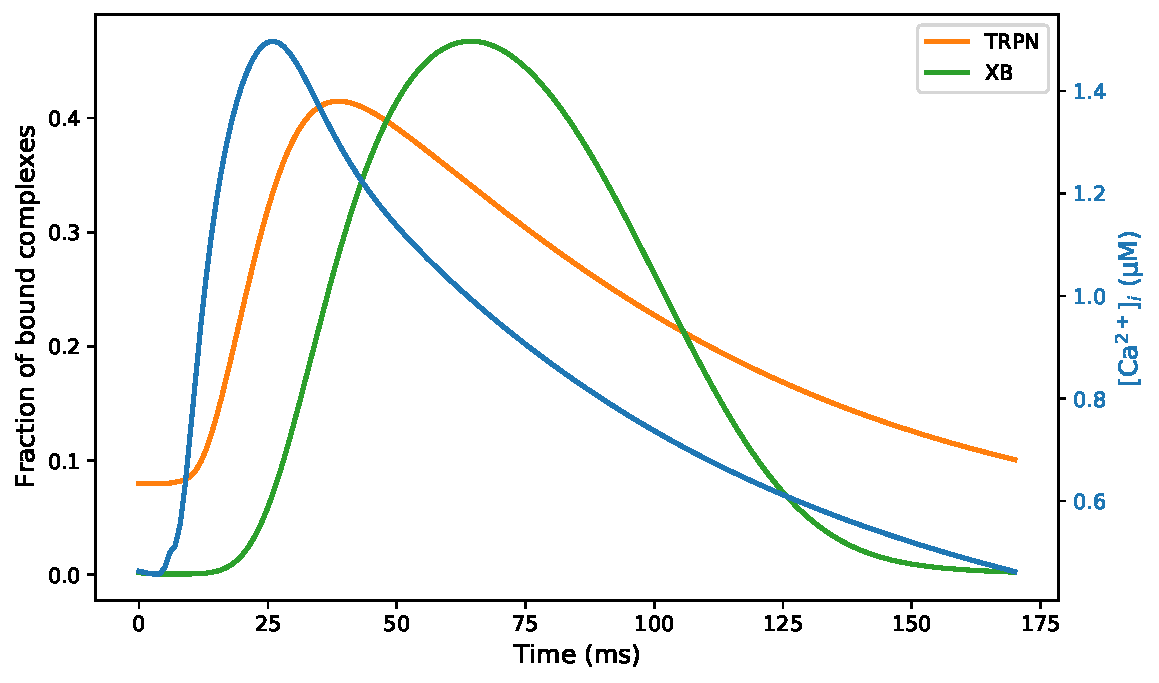
\includegraphics[width=0.8\textwidth]{figures/chapter02/Ca_TRPN_XB.pdf}
    \caption{Fraction of bound $\Ca$-TnC complexes (TRPN) and of bound cross-bridges (XB) as a function of time. The intracellular $\textrm{Ca}^{2+}$ concentration variation over time is also displayed on a different scale (blue).}
    \label{fig:catrpnxb}
\end{figure}

\vspace{0.2cm}
In the Land et al.~\cite{Land:2012} model, normalised active force is defined as:
%
\begin{equation}\label{eq:normforce}
    F_n = g(Q)\cdot h(\lambda)\cdot \text{XB}
\end{equation}

\noindent
where

\vspace{0.2cm}
\begin{tabular}{ll}
    $h(\lambda)$ & length-dependence factor \\
    $g(Q)$       & velocity-dependence factor
\end{tabular}

\vspace{0.2cm}\noindent
Normalised force (equation~\eqref{eq:normforce}) is then scaled to actual tension using a reference tension $\tref$ scaling coefficient that encapsulates the total number of cross-bridges and the fraction of cycling cross-bridges in the force-generating state for any given time:
%
\begin{equation}
    T = \tref\cdot F_n
\end{equation}


%
%
%
\subsection{Length-dependence}\label{sec:ch2lengthdependence}
The active tension dependence on sarcomere length was based on filament overlap modelling:
%
\begin{align}
    h'(\lambda) &= 1+\beta_0\,[\lambda+\min(\lambda,\,0.87)-1.87] \\
    h(\lambda) &= \max(0,\,h'(\min(\lambda,\,1.2)))
\end{align}

\noindent
where

\vspace{0.2cm}
\begin{tabular}{ll}
    $\beta_0$ & phenomenological tension length-dependence scaling factor
\end{tabular}

\vspace{0.2cm}\noindent
This results in a linear length dependence near resting sarcomere length and a twice as steep decrease in tension when the sarcomere length falls below the thick filament length (at $\lambda = 0.87$).

\vspace{0.2cm}
A phenomenological representation of the thin filament calcium sensitivity shift in a length-dependent manner is also included as an important mechanism of tension length-dependence. This is implemented by $\Caift$ in equation~\eqref{eq:landodesys1}, which is further taken to be:
%
\begin{equation}\label{eq:Caift}
    \Caift:=\Caif[1 + \beta_1(\lambda - 1)]
\end{equation}

\noindent
where

\vspace{0.2cm}
\begin{tabular}{ll}
    $\Caif$   & reference $\Ca$ thin filament sensitivity \\
    $\beta_1$ & phenomenological tension length-dependence scaling factor \\
    $\lambda$ & extension ratio along the fibre direction
\end{tabular}

\vspace{0.2cm}\noindent
At the resting sarcomere configuration ($\lambda=1$), length-dependence effects are not present, and no consequent shift in the calcium sensitivity is observed ($\Caift=\Caif$).


%
%
%
\subsection{Velocity-dependence}\label{sec:ch2velocitydependence}
To phenomenologically represent the tension development dependence on cross-bridge kinetics, the \emph{fading memory model} was employed as previously done in~\cite{Niederer:2006}, describing the velocity response as several strain-rate-dependent variables that decay with time. In particular, this model describes the relationship between tension and sarcomere sliding velocity by separating tension development into a non-linear static component and a linear time-dependent component, as described by the following two equations:
%
\begin{equation}
    \der{Q_i}{t} = A_i\,\der{\lambda}{t}-\alpha_i\,Q_i,\quad i=1,2
\end{equation}

\noindent
where

\vspace{0.2cm}
\begin{tabular}{ll}
    $A_i,\,i=1,2$      & parameters related to the viscous and elastic moduli \\
    $\alpha_i,\,i=1,2$ & parameters related to the frequencies
\end{tabular}

\vspace{0.2cm}\noindent
The effect $g(Q)$ seen in equation~\eqref{eq:normforce} on tension is given by an equation derived from the Hill force-velocity curve extended to model stretch and shortening in a symmetric way as done in~\cite{Niederer:2006}:
%
\begin{equation}
    g(Q) = \begin{cases}
        \dfrac{a\,Q+1}{1-Q}\qquad & Q\le 0 \\
        \dfrac{1+(a+2)\,Q}{1+Q}\qquad & Q>0
    \end{cases}\,,\quad\text{with}\quad Q := \sum_{i=1}^2 Q_i
\end{equation}

\noindent
where

\vspace{0.2cm}
\begin{tabular}{ll}
    $a$ & slope of the Hill force-velocity relationship
\end{tabular}

\vspace{0.2cm}\noindent
Land et al.~\cite{Land:2012} cell contraction model's main mechanisms are summarised in the schematic provided in Figure~\ref{fig:cellcontrschematic}.

\begin{figure}[ht!]
    \myfloatalign
    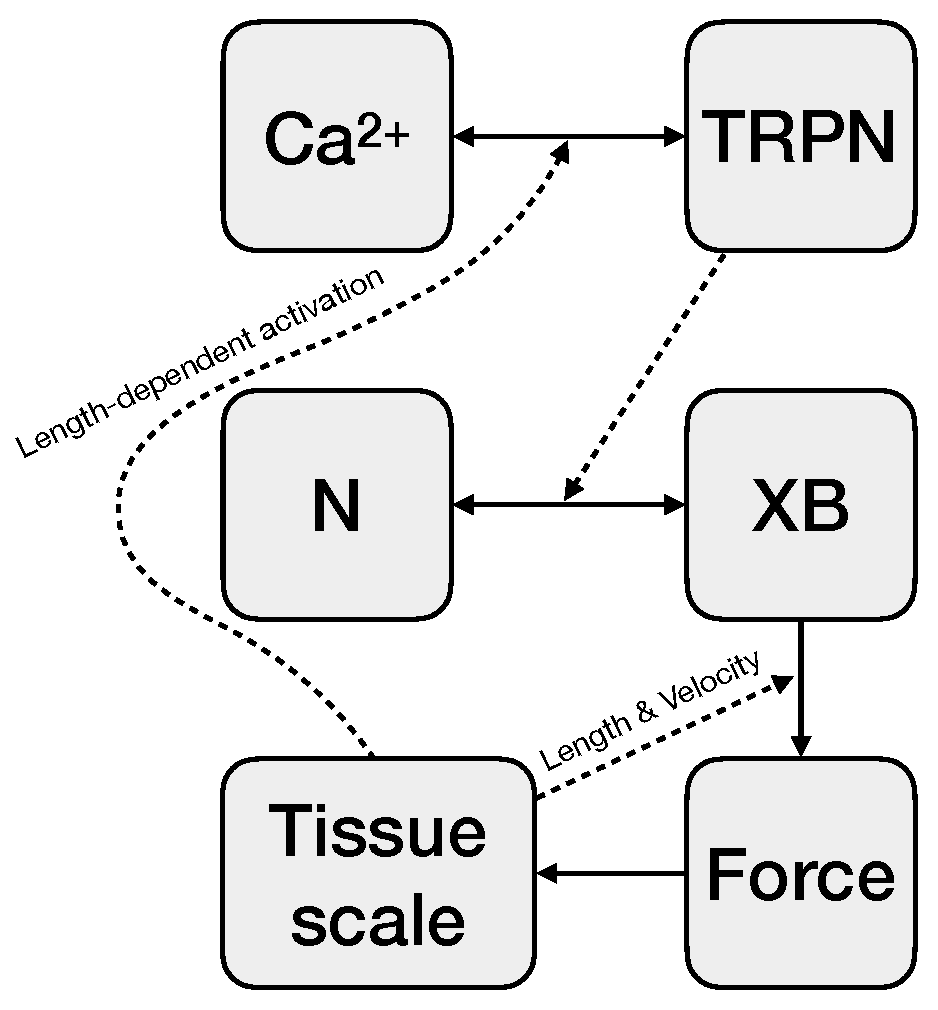
\includegraphics[width=0.66\textwidth]{figures/chapter02/cellular_contraction_land.pdf}
    \caption{Land et al.~\cite{Land:2012} cell contraction model schematic. $\Ca$ binds to TnC, and when the fraction of bound complexes (TRPN) reaches $\trpnf$, half of the maximum number of cross-bridges has passed from the non-permissive state (N) to the actively cycling state (XB). Generated active force, which directly depends on the fraction of formed cross-bridges, causes tissue contraction, which backwards modulates the force generation itself in a length- and velocity-dependent manner.}
    \label{fig:cellcontrschematic}
\end{figure}


%
%
%
\subsection{Uncoupling the binding and unbinding rates}\label{sec:ch2uncoupling_binding_and_unbinding_rates}
We wanted to uncouple the unbinding rate from the binding rate in the $\Ca$-TnC relationship. This was achieved by assigning a different function to parameter $\ktrpn$ according to whether this was multiplying the first term or the second term in equation~\eqref{eq:landodesys1}:
%
\begin{align}
    \frac{d\text{TRPN}}{dt} &=\ktrpn\left[\left(\frac{\Cai}{\Caift}\right)^{\ntrpn}(1-\trpn)-\trpn\right] \\
    &= \underbrace{\ktrpn}_{\kon}\left(\frac{\Cai}{\Caift}\right)^{\ntrpn}(1-\trpn)-\underbrace{\ktrpn}_{\koff}\trpn \\
    &= \kon\left(\frac{\Cai}{\Caift}\right)^{\ntrpn}(1-\trpn)-\koff\trpn \label{eq:landodesys1mod}
\end{align}

\vspace{0.2cm}\noindent
Both the $\Ca$-independent part ($\kon$) of the binding rate and the unbinding rate ($\koff$) were set to the same model baseline $\ktrpn$ value, although now it is possible to treat them as two different parameters. This will serve the purpose of understanding the individual contribution of each of them in the active tension generation.


%
%
%
\subsection{The force-calcium relationship}\label{sec:ch2theforcecalciumrelationship}
The steady-state solutions of Equations~\eqref{eq:landodesys1mod}--\eqref{eq:landodesys2} are:
%
\begin{equation}\label{eq:landodesys1_ss}
    \trpn_{ss} = \dfrac{\left(\dfrac{\Cai}{\Caift}\right)^{\ntrpn}}{\dfrac{\koff}{\kon}+\left(\dfrac{\Cai}{\Caift}\right)^{\ntrpn}}
\end{equation}
%
\begin{equation}\label{eq:landodesys2_ss}
    \xb_{ss} = \frac{(\trpn)^{\nxb}}{(\trpnf)^{\nxb}+(\trpn)^{\nxb}}
\end{equation}

\noindent
In the case of isometric force studies, the length- ($h(\lambda)$) and velocity- ($g(Q)$) dependence terms equal to $1$, and the steady-state force is given by:
%
\begin{equation}\label{eq:landssforce}
    F = \tref\cdot \xb_{ss}
\end{equation}

\noindent
Equation~\eqref{eq:landssforce} can be re-written in a more classical form as
%
\begin{equation}\label{eq:forcess}
    \frac{F}{F_0} = \frac{x^{h(x)}}{1+x^{h(x)}}\,,\quad\text{with}\quad x:=\frac{\Cai}{\ecf}
\end{equation}

\noindent
where

\vspace{0.2cm}
\begin{tabular}{ll}
    $F_0$  & reference force ($=\tref$) \\
    $h(x)$ & Hill coefficient \\
    $\ecf$ & half-maximal effective concentration
\end{tabular}

\vspace{0.2cm}\noindent
The Hill coefficient $h(x)$ has the following form:
%
\begin{equation}
    h(x) = \nxb\left[\ntrpn-\log_{x}{\left(1-\trpnf(1-x^{\ntrpn})\right)}\right]
\end{equation}

\noindent
while the half-maximal effective concentration $\ecf$ is given as a function of five model parameters:
%
\begin{equation}\label{eq:ec50}
    \ecf = \Caift\left(\frac{\koff}{\kon}\frac{\trpnf}{1-\trpnf}\right)^{1/\ntrpn}
\end{equation}

By construction, the Land et al.~\cite{Land:2012} model has a biphasic Hill coefficient. To simplify the analysis, we approximated the steady-state force by characterising $F$ using a single Hill coefficient value $h$ defined as the slope at half-maximal activation:
%
\begin{equation}\label{eq:h}
    h := \lim_{x\to1}h(x) = \nxb\ntrpn(1-\trpnf)
\end{equation}

\noindent
As a result, the Hill coefficient does not depend on $\Cai$ and is a function of three model parameters. Using logarithmically-spaced calcium values, equation~\eqref{eq:forcess} becomes
%
\begin{align}\label{eq:FpCa}
    & \frac{F}{F_0} = \frac{1}{1+10^{h(\pCaf-\pCa)}}\,,\quad\text{with} \\
    & \pCa:=-\log{\Cai} \\
    & \pCaf:=-\log{\ecf}
\end{align}

\noindent
Equation~\eqref{eq:FpCa} takes the name of \textit{force-pCa} (\acs{F-pCa}) \textit{curve}.


%
%
%
\section{Anatomy model}\label{sec:ch2anatomy}
Rat biventricular anatomy was represented \textit{in silico} by a cubic Hermite finite element mesh. This was generated using an automatic service for ventricular cardiac meshes personalisation developed by Lamata et al.~\cite{Lamata:2011, Lamata:2014}.

\vspace{0.2cm}
The mesh customisation pipeline starts from a binary image, which in general corresponds to a segmentation obtained from heart medical images (e.g. magnetic resonance images). An idealised template mesh composed of truncated ellipsoids is then tailored to the binary mask provided, and image registration is performed to assess the deformation field from template to real anatomy. During this step, the user can choose the so-called \textit{level of detail} (\acs{LoD}), which gives a trade-off between fitting accuracy and numerical stability. The LoD ranges from $1$ (coarse and most stable) to $5$ (accurate but less likely to be stable). After having calculated the warping function by image registration, this is used to map the template mesh to the deformed space using a variational technique. The last step of the pipeline involves enhancing the quality of the mesh by improving the regularity of each element by linearising internal nodes transmural positions with no loss of accuracy.

\vspace{0.2cm}
Rule-based fibres~\cite{Bayer:2012}, along with the generated meshes, complemented the anatomical description of the rat heart. We used a transmural variation of $\SI{-60}{\degree}$ to $\SI{80}{\degree}$ from epicardium to endocardium.


%
%
%
\section{Tissue model}\label{sec:ch2tissuemodel}
We modelled passive material properties using the transversely isotropic cardiac strain energy function proposed by Guccione et al.~\cite{Guccione:1991}:
%
\begin{align}\label{eq:guccstrainenergy}
    &W = W_g(\mathbf{E})\,,\quad\text{with} \\
    &W_g(\mathbf{E}) := \frac{1}{2}\,C_1\,(e^{Q(\mathbf{E})}-1) \\
    &Q(\mathbf{E}) := b_f E_{\text{ff}}^2 + b_{ft}(2E_{\text{fs}}^2+2E_{\text{fn}}^2) + b_t(E_{\text{ss}}^2+E_{\text{nn}}^2+2\,E_{\text{sn}}^2)
\end{align}

\noindent
where

\vspace{0.2cm}
\begin{tabular}{ll}
    $\mathbf{E}$ & Green strain tensor (introduced in Section~\ref{sec:tissue_mech_math_modelling}) \\
    $C_1$ & scaling coefficient (representing an overall tissue stiffness) \\
    $b_f,\,b_{ft},\,b_t$ & tissue mechanical response in the fibre, \\ & fibre-transverse shear and transverse planes \\
\end{tabular}

\vspace{0.2cm}\noindent
Moreover, cardiac tissue was assumed to be fully incompressible. This was enforced by expanding the strain-energy function in equation~\eqref{eq:guccstrainenergy} with a Lagrange multiplier scheme, in combination with an incompressibility penalty to improve stability of mechanics simulations~\cite{Land:2012*a, Land:2015*b}:
%
\begin{align}\label{eq:landstrainenergy}
    &W = W_g(\mathbf{E}) - p(J - 1) + \frac{\kappa}{2}(J - 1)^2\,,\quad\text{with}\quad J:=\text{det}(\mathbf{F}) \\
    &\text{and with constraint:}\quad J=1
\end{align}

\noindent
where

\vspace{0.2cm}
\begin{tabular}{ll}
    $p$ & hydrostatic pressure \\
    $\kappa$ & penalty parameter \\
    $\mathbf{F}$ & deformation gradient tensor (introduced in Section~\ref{sec:tissue_mech_math_modelling})
\end{tabular}


%
%
%
\section{Electrical activation}\label{sec:ch2electricalactivation}
The calcium transient was assumed not to vary spatially, and it homogeneously activated contraction throughout the ventricular walls. Previous heart models
have shown that heterogeneous activation patterns have negligible impact in the small rat heart \todo{REF}, and so activation was assumed instantaneous for simplicity and to improve computational tractability.


%
%
%
\section{Boundary conditions}\label{sec:ch2boundaryconditions}
We applied spatial boundary conditions to the mesh throughout the mechanics solution process. Specifically, we constrained all the ventricles basal plane mesh nodes along the apex-base axis and allowed no movement along any direction for one node on the interior LV wall. This constraint prevented free rotation and translation without limiting the deformation~\cite{Land:2012}.

\vspace{0.2cm}
We also set haemodynamic boundary conditions to control blood flow and pressures at the computational domain boundaries, thereby coupling the biventricular heart with the rest of the body circulatory system. We used a three-element Windkessel model~\cite{Westerhof:1971} to regulate ejection, and we used the Windkessel model generalised formulation (equation~\eqref{eq:windkgeneral}) to regulate the other phases of the cardiac cycle, namely initial preload filling, isovolumetric contraction, isovolumetric relaxation and diastolic filling, as described in Section~\ref{sec:hemodynamics_math_modelling}. The RV boundary condition pressures (atrial and pulmonary artery) were set to be $1/3$ of the equivalent LV values \todo{REF}. The RV Windkessel parameters were scaled to be equal to $R/3$, $Z/3$, $3C$ from the reference LV Windkessel parameter set ($R$, $Z$, $C$).


%
%
%
\section{Simulation protocol}\label{sec:ch2simulationprotocol}
The whole-organ complete cardiac cycle was simulated using the protocol described in~\cite{Land:2012, Land:2012*a, Land:2015}. Briefly, dynamic changes in the LV and RV cavities' boundary conditions were cyclically applied. During diastole, a fixed atrial preload pressure and filling resistance was applied. At activation, the cavity boundary conditions were switched to an isovolumetric constraint in both chambers. When each chamber reached pre-set aortic and pulmonary artery pressures, a three-element Windkessel model boundary condition was applied to each chamber to represent the aortic and pulmonary artery afterload. Once each chamber stopped ejecting, an isovolumetric boundary condition was applied to represent isovolumetric relaxation. Once the cavity pressure fell below its respective atrial pressure, the heart returned to the diastolic cavity boundary conditions to complete the PV loop.


%
%
%
\section{Summary}\label{sec:ch2summary}
We modelled the rat heart using a $3$D biventricular contraction mechanics model. Cellular electrophysiology was simulated using the Gattoni et al.~\cite{Gattoni:2016} model of rat LV myocytes at $\SI{37}{\celsius}$ and $\SI{6}{\hertz}$ pacing frequency. Active tension generation was described using the Land et al.~\cite{Land:2012*a} model of sarcomere contraction. LV and RV anatomy was represented by a cubic Hermite finite element mesh~\cite{Lamata:2011}. Rule-based fibres~\cite{Bayer:2012} were included with a transmural variation of $\SI{-60}{\degree}$ to $\SI{80}{\degree}$ from epicardium to endocardium. Passive material properties were modelled using the Guccione transversely isotropic cardiac strain energy function~\cite{Guccione:1991}, combined with a Lagrange multiplier scheme and a penalty term~\cite{Land:2012*a, Land:2015*b}. The $\Ca$ transient was assumed not to vary spatially, and it homogeneously activated contraction throughout the ventricular walls. Spatial boundary conditions were applied by constraining the movement of specific mesh nodes, and haemodynamic boundary conditions were described by a generalised three-element Windkessel model~\cite{Westerhof:1991}.